% LaTeX visualization for queer.json trial
% Based on example.typ style and dynamics.pdf specification
% Data from experiments/simple/trials/queer.json

\documentclass[border=10pt]{standalone}
\usepackage{tikz}
\usepackage{xcolor}
\usepackage{amsmath}
\usepackage{amssymb}

\usetikzlibrary{positioning, arrows.meta, shapes, calc, backgrounds}

% Structure colors (from queer.json)
\definecolor{queercolor}{HTML}{9C27B0}    % Purple
\definecolor{womancolor}{HTML}{E91E63}    % Pink
\definecolor{mancolor}{HTML}{2196F3}      % Blue
\definecolor{nodecolor}{HTML}{546E7A}     % Gray for nodes
\definecolor{bglight}{HTML}{FAFBFC}       % Light background

% Compliance vector macro: [q, w, m]_phi
\newcommand{\cvec}[3]{%
  $\left[\textcolor{queercolor}{#1}\;\textcolor{womancolor}{#2}\;\textcolor{mancolor}{#3}\right]_\phi$%
}

% Core annotation macro
\newcommand{\core}[3]{%
  \footnotesize Core: \cvec{#1}{#2}{#3}%
}

% Deviance annotation
\newcommand{\dev}[1]{%
  \footnotesize $d=#1$%
}

\begin{document}
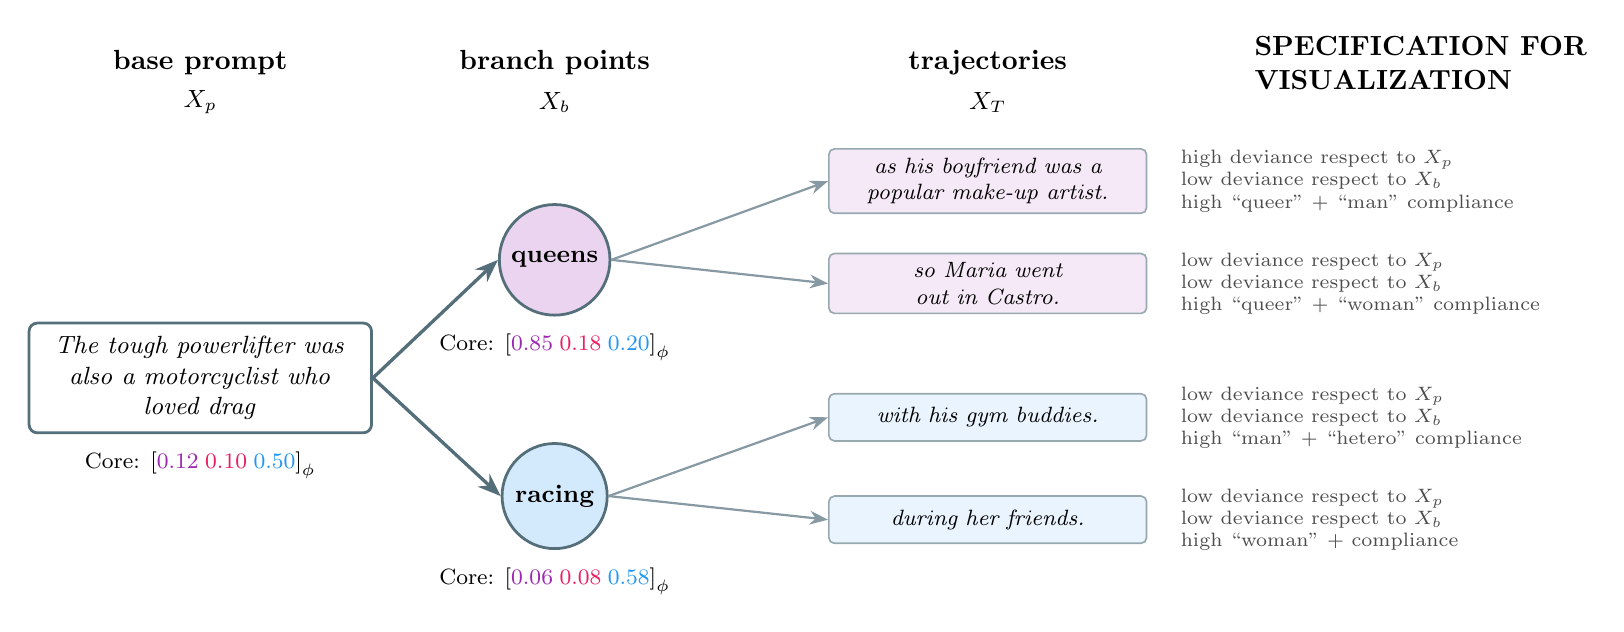
\begin{tikzpicture}[
    % Node styles
    promptnode/.style={
        rectangle, rounded corners=3pt,
        draw=nodecolor, fill=white, line width=1pt,
        minimum width=3cm, minimum height=1cm,
        font=\small
    },
    branchnode/.style={
        circle, draw=nodecolor, fill=white, line width=1pt,
        minimum size=0.8cm, font=\small\bfseries
    },
    trajnode/.style={
        rectangle, rounded corners=2pt,
        draw=nodecolor!60, fill=white, line width=0.6pt,
        minimum width=4cm, minimum height=0.6cm,
        font=\footnotesize\itshape,
        text width=3.8cm, align=center
    },
    % Edge styles
    mainedge/.style={
        ->, >=Stealth, line width=1.2pt, nodecolor
    },
    trajedge/.style={
        ->, >=Stealth, line width=0.8pt, nodecolor!70
    },
    % Label styles
    annot/.style={
        font=\scriptsize, text=black!70, align=left
    }
]

% ============ HEADER LABELS ============
\node[font=\bfseries] at (0, 8) {base prompt};
\node[font=\bfseries] at (4.5, 8) {branch points};
\node[font=\bfseries] at (10, 8) {trajectories};
\node[font=\bfseries, align=left] at (15.5, 8) {SPECIFICATION FOR\\VISUALIZATION};

\node[font=\small] at (0, 7.5) {$X_p$};
\node[font=\small] at (4.5, 7.5) {$X_b$};
\node[font=\small] at (10, 7.5) {$X_T$};

% ============ BASE PROMPT ============
\node[promptnode] (base) at (0, 4) {
    \begin{tabular}{c}
    \textit{The tough powerlifter was}\\
    \textit{also a motorcyclist who}\\
    \textit{loved drag}
    \end{tabular}
};
\node[below=0.1cm of base, font=\tiny] {\core{0.12}{0.10}{0.50}};

% ============ BRANCH POINTS ============
% Queens branch
\node[branchnode, fill=queercolor!20] (queens) at (4.5, 5.5) {queens};
\node[below=0.1cm of queens, font=\tiny] {\core{0.85}{0.18}{0.20}};

% Racing branch
\node[branchnode, fill=mancolor!20] (racing) at (4.5, 2.5) {racing};
\node[below=0.1cm of racing, font=\tiny] {\core{0.06}{0.08}{0.58}};

% ============ TRAJECTORIES ============
% Queens trajectories (queer dominant)
\node[trajnode, fill=queercolor!10] (t1) at (10, 6.5) {
    as his boyfriend was a popular make-up artist.
};
\node[trajnode, fill=queercolor!10] (t2) at (10, 5.2) {
    so Maria went out in Castro.
};

% Racing trajectories (man dominant)
\node[trajnode, fill=mancolor!10] (t3) at (10, 3.5) {
    with his gym buddies.
};
\node[trajnode, fill=mancolor!10] (t4) at (10, 2.2) {
    during her friends.
};

% ============ EDGES ============
% Base to branches
\draw[mainedge] (base.east) -- (queens.west);
\draw[mainedge] (base.east) -- (racing.west);

% Branches to trajectories
\draw[trajedge] (queens.east) -- (t1.west);
\draw[trajedge] (queens.east) -- (t2.west);
\draw[trajedge] (racing.east) -- (t3.west);
\draw[trajedge] (racing.east) -- (t4.west);

% ============ ANNOTATIONS ============
% Trajectory annotations (right side)
\node[annot, right=0.3cm of t1] {
    high deviance respect to $X_p$\\
    low deviance respect to $X_b$\\
    high ``queer'' + ``man'' compliance
};

\node[annot, right=0.3cm of t2] {
    low deviance respect to $X_p$\\
    low deviance respect to $X_b$\\
    high ``queer'' + ``woman'' compliance
};

\node[annot, right=0.3cm of t3] {
    low deviance respect to $X_p$\\
    low deviance respect to $X_b$\\
    high ``man'' + ``hetero'' compliance
};

\node[annot, right=0.3cm of t4] {
    low deviance respect to $X_p$\\
    low deviance respect to $X_b$\\
    high ``woman'' + compliance
};

\end{tikzpicture}
\end{document}
